\documentclass[leqno, 12pt]{article}
\usepackage{tikz}
\usepackage{amsmath}
\usepackage{ulem}
\usetikzlibrary{angles,quotes,intersections,arrows.meta,calc}
\usepackage[a4paper, portrait, margin=1cm]{geometry}
\usepackage{multicol}
\usepackage{fancyhdr}

\def \HeadingAnswers {\section*{\Large Name: \underline{\hspace{8cm}} \hfill Date: \underline{\hspace{3cm}}} \vspace{-3mm}
{Parallel lines : Answers} \vspace{1pt}\hrule}

% raise footer with page number; no header
\fancypagestyle{myfancypagestyle}{
  \fancyhf{}% clear all header and footer fields
  \renewcommand{\headrulewidth}{0pt} % no rule under header
  \fancyfoot[C] {\thepage} \setlength{\footskip}{14.5pt} % raise page number allowed min 14.5pt
}
\pagestyle{myfancypagestyle}  % apply myfancypagestyle

\newcounter{minipagecount}

\begin{document}
\HeadingAnswers
\begin{multicols}{2}


\begin{equation}
  \text{f} = \text{71}^\circ
  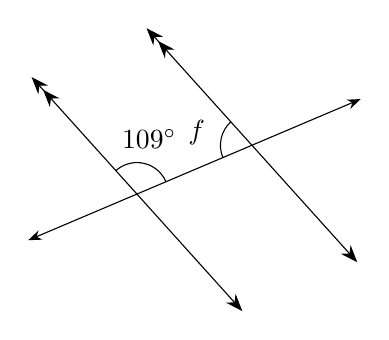
\begin{tikzpicture}[scale=1.0, baseline=(current bounding box.north)]
    \begin{scope}[rotate=23]
      % Draw the first line
      \draw[<->>, >={Stealth[scale=1.3]}, name path=P1] (0, 0) -- (-1.3022726178286266, 3.7820743023972674);
      % Draw the second line with the calculated offsets
      \draw[<->>, >={Stealth[scale=1.3]}, name path=P2] (1.586431021780006, 0) -- (0.28415840395137937, 3.7820743023972674);
      % Draw the transversal through the middle of the parallel lines
      \draw[<->, >=Stealth, name path=P3] (-2.1511363089143134, 1.8910371511986337) -- (2.435294712865693, 1.8910371511986337);
      \path [name intersections={of=P1 and P3,by=A}];
      \path [name intersections={of=P2 and P3,by=B}];
      % Draw the angle
      \coordinate (p1s) at (0, 0);
      \coordinate (p1e) at (-1.3022726178286266, 3.7820743023972674);
      \coordinate (p2s) at (1.586431021780006, 0);
      \coordinate (p2e) at (0.28415840395137937, 3.7820743023972674);
      \coordinate (ts) at (-2.1511363089143134, 1.8910371511986337);
      \coordinate (te) at (2.435294712865693, 1.8910371511986337);
      \draw pic["$f$", draw=black, -, angle eccentricity=1.8, angle radius=0.4cm] {angle=p2e--B--ts};
\draw pic["$109^\circ$", draw=black, -, angle eccentricity=1.8, angle radius=0.4cm] {angle=te--A--p1e};

    \end{scope}
  \end{tikzpicture}
\end{equation}\vspace{1cm}
\begin{equation}
  \text{a} = \text{64}^\circ
  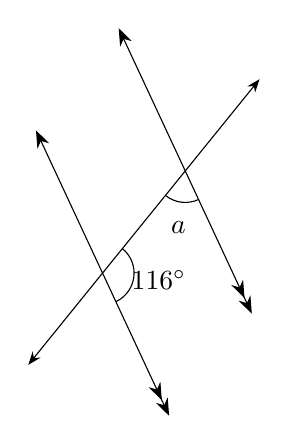
\begin{tikzpicture}[scale=1.0, baseline=(current bounding box.north)]
    \begin{scope}[rotate=231]
      % Draw the first line
      \draw[<->>, >={Stealth[scale=1.3]}, name path=P1] (0, 0) -- (1.7534845871563098, 3.595176185196668);
      % Draw the second line with the calculated offsets
      \draw[<->>, >={Stealth[scale=1.3]}, name path=P2] (1.6689029107127833, 0) -- (3.422387497869093, 3.595176185196668);
      % Draw the transversal through the middle of the parallel lines
      \draw[<->, >=Stealth, name path=P3] (-0.6232577064218452, 1.797588092598334) -- (4.045645204290938, 1.797588092598334);
      \path [name intersections={of=P1 and P3,by=A}];
      \path [name intersections={of=P2 and P3,by=B}];
      % Draw the angle
      \coordinate (p1s) at (0, 0);
      \coordinate (p1e) at (1.7534845871563098, 3.595176185196668);
      \coordinate (p2s) at (1.6689029107127833, 0);
      \coordinate (p2e) at (3.422387497869093, 3.595176185196668);
      \coordinate (ts) at (-0.6232577064218452, 1.797588092598334);
      \coordinate (te) at (4.045645204290938, 1.797588092598334);
      \draw pic["$a$", draw=black, -, angle eccentricity=1.8, angle radius=0.4cm] {angle=te--A--p1e};
\draw pic["$116^\circ$", draw=black, -, angle eccentricity=1.8, angle radius=0.4cm] {angle=p2e--B--ts};

    \end{scope}
  \end{tikzpicture}
\end{equation}\vspace{1cm}
\begin{equation}
  \text{f} = \text{35}^\circ
  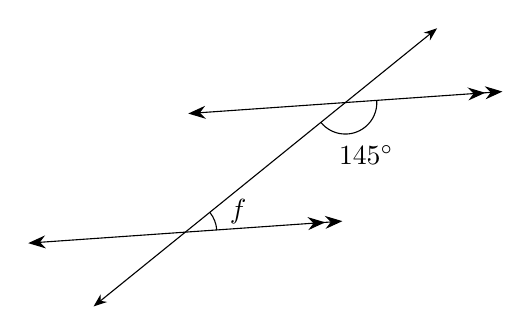
\begin{tikzpicture}[scale=1.0, baseline=(current bounding box.north)]
    \begin{scope}[rotate=219]
      % Draw the first line
      \draw[<->>, >={Stealth[scale=1.3]}, name path=P1] (0, 0) -- (-3.2766081771559676, 2.2943057454041837);
      % Draw the second line with the calculated offsets
      \draw[<->>, >={Stealth[scale=1.3]}, name path=P2] (2.6151701934316476, 0) -- (-0.66143798372432, 2.2943057454041837);
      % Draw the transversal through the middle of the parallel lines
      \draw[<->, >=Stealth, name path=P3] (-3.1383040885779834, 1.1471528727020919) -- (2.4768661048536633, 1.1471528727020919);
      \path [name intersections={of=P1 and P3,by=A}];
      \path [name intersections={of=P2 and P3,by=B}];
      % Draw the angle
      \coordinate (p1s) at (0, 0);
      \coordinate (p1e) at (-3.2766081771559676, 2.2943057454041837);
      \coordinate (p2s) at (2.6151701934316476, 0);
      \coordinate (p2e) at (-0.66143798372432, 2.2943057454041837);
      \coordinate (ts) at (-3.1383040885779834, 1.1471528727020919);
      \coordinate (te) at (2.4768661048536633, 1.1471528727020919);
      \draw pic["$f$", draw=black, -, angle eccentricity=1.8, angle radius=0.4cm] {angle=p2e--B--ts};
\draw pic["$145^\circ$", draw=black, -, angle eccentricity=1.8, angle radius=0.4cm] {angle=te--A--p1e};

    \end{scope}
  \end{tikzpicture}
\end{equation}\vspace{1cm}
\begin{equation}
  \text{g} = \text{97}^\circ
  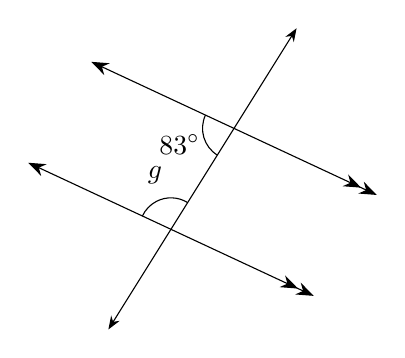
\begin{tikzpicture}[scale=1.0, baseline=(current bounding box.north)]
    \begin{scope}[rotate=238]
      % Draw the first line
      \draw[<->>, >={Stealth[scale=1.3]}, name path=P1] (0, 0) -- (-0.48747737362058946, 3.9701846065652884);
      % Draw the second line with the calculated offsets
      \draw[<->>, >={Stealth[scale=1.3]}, name path=P2] (1.5112647381882724, 0) -- (1.023787364567683, 3.9701846065652884);
      % Draw the transversal through the middle of the parallel lines
      \draw[<->, >=Stealth, name path=P3] (-1.7437386868102949, 1.9850923032826442) -- (2.767526051377978, 1.9850923032826442);
      \path [name intersections={of=P1 and P3,by=A}];
      \path [name intersections={of=P2 and P3,by=B}];
      % Draw the angle
      \coordinate (p1s) at (0, 0);
      \coordinate (p1e) at (-0.48747737362058946, 3.9701846065652884);
      \coordinate (p2s) at (1.5112647381882724, 0);
      \coordinate (p2e) at (1.023787364567683, 3.9701846065652884);
      \coordinate (ts) at (-1.7437386868102949, 1.9850923032826442);
      \coordinate (te) at (2.767526051377978, 1.9850923032826442);
      \draw pic["$g$", draw=black, -, angle eccentricity=1.8, angle radius=0.4cm] {angle=ts--B--p2s};
\draw pic["$83^\circ$", draw=black, -, angle eccentricity=1.8, angle radius=0.4cm] {angle=p1s--A--te};

    \end{scope}
  \end{tikzpicture}
\end{equation}\vspace{1cm}
\begin{equation}
  \text{a} = \text{48}^\circ
  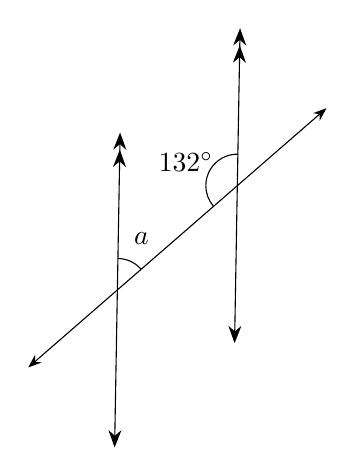
\begin{tikzpicture}[scale=1.0, baseline=(current bounding box.north)]
    \begin{scope}[rotate=41]
      % Draw the first line
      \draw[<->>, >={Stealth[scale=1.3]}, name path=P1] (0, 0) -- (2.676522425435433, 2.972579301909577);
      % Draw the second line with the calculated offsets
      \draw[<->>, >={Stealth[scale=1.3]}, name path=P2] (2.018449094409564, 0) -- (4.694971519844997, 2.972579301909577);
      % Draw the transversal through the middle of the parallel lines
      \draw[<->, >=Stealth, name path=P3] (-0.16173878728228352, 1.4862896509547885) -- (4.856710307127281, 1.4862896509547885);
      \path [name intersections={of=P1 and P3,by=A}];
      \path [name intersections={of=P2 and P3,by=B}];
      % Draw the angle
      \coordinate (p1s) at (0, 0);
      \coordinate (p1e) at (2.676522425435433, 2.972579301909577);
      \coordinate (p2s) at (2.018449094409564, 0);
      \coordinate (p2e) at (4.694971519844997, 2.972579301909577);
      \coordinate (ts) at (-0.16173878728228352, 1.4862896509547885);
      \coordinate (te) at (4.856710307127281, 1.4862896509547885);
      \draw pic["$a$", draw=black, -, angle eccentricity=1.8, angle radius=0.4cm] {angle=te--A--p1e};
\draw pic["$132^\circ$", draw=black, -, angle eccentricity=1.8, angle radius=0.4cm] {angle=p2e--B--ts};

    \end{scope}
  \end{tikzpicture}
\end{equation}\vspace{1cm}
\begin{equation}
  \text{a} = \text{134}^\circ
  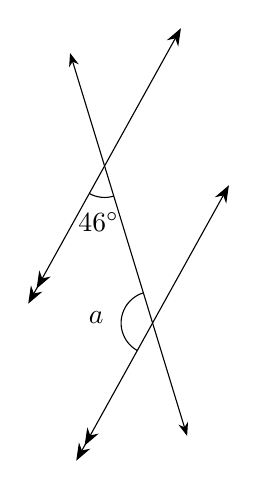
\begin{tikzpicture}[scale=1.0, baseline=(current bounding box.north)]
    \begin{scope}[rotate=107]
      % Draw the first line
      \draw[<->>, >={Stealth[scale=1.3]}, name path=P1] (0, 0) -- (-2.7786334818359895, 2.8773592013546043);
      % Draw the second line with the calculated offsets
      \draw[<->>, >={Stealth[scale=1.3]}, name path=P2] (2.0852453865250182, 0) -- (-0.6933880953109712, 2.8773592013546043);
      % Draw the transversal through the middle of the parallel lines
      \draw[<->, >=Stealth, name path=P3] (-2.889316740917995, 1.4386796006773022) -- (2.1959286456070237, 1.4386796006773022);
      \path [name intersections={of=P1 and P3,by=A}];
      \path [name intersections={of=P2 and P3,by=B}];
      % Draw the angle
      \coordinate (p1s) at (0, 0);
      \coordinate (p1e) at (-2.7786334818359895, 2.8773592013546043);
      \coordinate (p2s) at (2.0852453865250182, 0);
      \coordinate (p2e) at (-0.6933880953109712, 2.8773592013546043);
      \coordinate (ts) at (-2.889316740917995, 1.4386796006773022);
      \coordinate (te) at (2.1959286456070237, 1.4386796006773022);
      \draw pic["$a$", draw=black, -, angle eccentricity=1.8, angle radius=0.4cm] {angle=te--A--p1e};
\draw pic["$46^\circ$", draw=black, -, angle eccentricity=1.8, angle radius=0.4cm] {angle=p2e--B--ts};

    \end{scope}
  \end{tikzpicture}
\end{equation}\vspace{1cm}
\begin{equation}
  \text{g} = \text{89}^\circ
  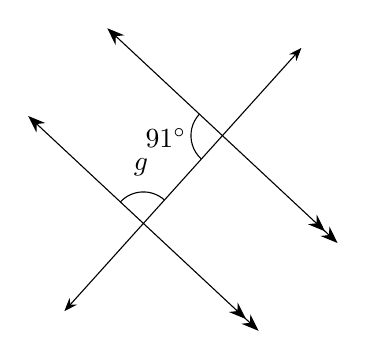
\begin{tikzpicture}[scale=1.0, baseline=(current bounding box.north)]
    \begin{scope}[rotate=228]
      % Draw the first line
      \draw[<->>, >={Stealth[scale=1.3]}, name path=P1] (0, 0) -- (0.0698096257491344, 3.999390780625565);
      % Draw the second line with the calculated offsets
      \draw[<->>, >={Stealth[scale=1.3]}, name path=P2] (1.5002284920658615, 0) -- (1.5700381178149958, 3.999390780625565);
      % Draw the transversal through the middle of the parallel lines
      \draw[<->, >=Stealth, name path=P3] (-1.465095187125433, 1.9996953903127825) -- (3.0351333049404285, 1.9996953903127825);
      \path [name intersections={of=P1 and P3,by=A}];
      \path [name intersections={of=P2 and P3,by=B}];
      % Draw the angle
      \coordinate (p1s) at (0, 0);
      \coordinate (p1e) at (0.0698096257491344, 3.999390780625565);
      \coordinate (p2s) at (1.5002284920658615, 0);
      \coordinate (p2e) at (1.5700381178149958, 3.999390780625565);
      \coordinate (ts) at (-1.465095187125433, 1.9996953903127825);
      \coordinate (te) at (3.0351333049404285, 1.9996953903127825);
      \draw pic["$g$", draw=black, -, angle eccentricity=1.8, angle radius=0.4cm] {angle=ts--B--p2s};
\draw pic["$91^\circ$", draw=black, -, angle eccentricity=1.8, angle radius=0.4cm] {angle=p1s--A--te};

    \end{scope}
  \end{tikzpicture}
\end{equation}\vspace{1cm}
\begin{equation}
  \text{a} = \text{35}^\circ
  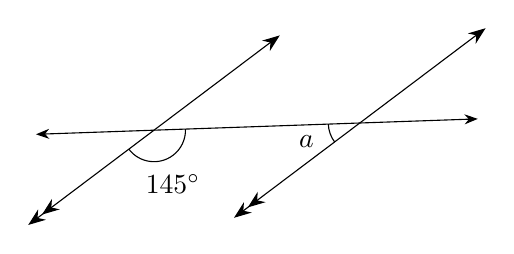
\begin{tikzpicture}[scale=1.0, baseline=(current bounding box.north)]
    \begin{scope}[rotate=182]
      % Draw the first line
      \draw[<->>, >={Stealth[scale=1.3]}, name path=P1] (0, 0) -- (3.276608177155967, 2.294305745404184);
      % Draw the second line with the calculated offsets
      \draw[<->>, >={Stealth[scale=1.3]}, name path=P2] (2.615170193431647, 0) -- (5.891778370587614, 2.294305745404184);
      % Draw the transversal through the middle of the parallel lines
      \draw[<->, >=Stealth, name path=P3] (0.13830408857798382, 1.147152872702092) -- (5.7534742820096305, 1.147152872702092);
      \path [name intersections={of=P1 and P3,by=A}];
      \path [name intersections={of=P2 and P3,by=B}];
      % Draw the angle
      \coordinate (p1s) at (0, 0);
      \coordinate (p1e) at (3.276608177155967, 2.294305745404184);
      \coordinate (p2s) at (2.615170193431647, 0);
      \coordinate (p2e) at (5.891778370587614, 2.294305745404184);
      \coordinate (ts) at (0.13830408857798382, 1.147152872702092);
      \coordinate (te) at (5.7534742820096305, 1.147152872702092);
      \draw pic["$a$", draw=black, -, angle eccentricity=1.8, angle radius=0.4cm] {angle=te--A--p1e};
\draw pic["$145^\circ$", draw=black, -, angle eccentricity=1.8, angle radius=0.4cm] {angle=p2e--B--ts};

    \end{scope}
  \end{tikzpicture}
\end{equation}\vspace{1cm}

\end{multicols}
\end{document}

